\taskpic{ Внутри $U$--образной трубки массы $M$, лежащей на столе,
  находится нерастяжимая нить массы $m$. В начальный момент в каждом
  колене трубки находится по половине нити, а сама трубка
  движется. Нить в трубке движется так, что скорость конца $A$ нити
  равна $v$, а скорость конца $B$ --- нулю. С какой скоростью будет
  двигаться трубка, когда нить вылетит из неё? Трением
  пренебречь. Радиус изгиба трубки считать очень малым. }
{
  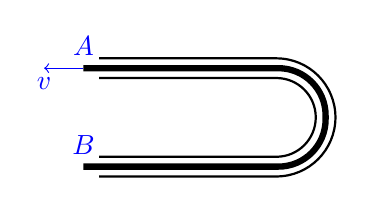
\begin{tikzpicture}
    \draw[thick,rounded corners=0.75cm] (0.5,0) -- (3.5,0) -- (3.5,1.5)
    -- (0.5,1.5);
    \draw[thick,rounded corners=0.5cm] (0.5,0.25) -- (3.25,0.25) --
    (3.25,1.25) -- (0.5,1.25);
    \draw[line width=0.08cm, rounded corners=0.6cm] (0.3,0.125)
    node[above,blue] {$B$} -- (3.375,0.125) -- (3.375,1.375) --
    (0.3,1.375) node[above,blue] {$A$};
    \draw[blue,->] (0.3,1.375) -- ++(-0.5,0) node[below] {$v$};
  \end{tikzpicture}
}
% Новосиб, 1.103
